\documentclass[11pt,a4paper]{article}
\usepackage[left=2cm,text={17cm,25cm},top=2cm]{geometry}
\usepackage[T1]{fontenc}
\usepackage[czech]{babel}
\usepackage[utf8]{inputenc}
\usepackage{url}
\usepackage{graphicx}
\usepackage{pdfpages}
\usepackage{algorithmicx}
\graphicspath{ {img/} }

\begin{document}

\begin{center}
	\LARGE{Paralelní a distribuované algoritmy -- dokumentace k projektu 2}\\
	\large{Vysoké učení technické v Brně}
	\vspace{0.2cm}

	Petr Stehlík <xstehl14@stud.fit.vutbr.cz>     \today

\end{center}

\section{Zadání}

Cílem projektu byla implementace algoritmu mesh multiplication, který byl prezentován během přednášek. Běh a kompilace programu je zprostředkován pomocí skriptu \texttt{test.sh}. Implementace využívá knihovny Open MPI.

\section{Rozbor a analýza algoritmu}

Mesh multiplication je algoritmus pro součin dvou matic $A(m,n)$ a $B(n,k)$, kde výsledkem je matice $C (m,k) = AB$, kde $C_{ij} = \sum\limits_{s=1}^n a_{is} * b_{sj}$, kde $1 \leq i \leq m, 1 \leq j \leq k$. Algoritmus pro jednoduchost budeme analyzovat a popisovat na čtvercových maticích, avšak algoritmus je aplikovatelný i na obdélníkové matice jak jsou definovány výše.

Procesory jsou propojeny v dvourozměrné mřízce a lineárně spojeny se svými nejbližšími sousedy. Schéma zapojení procesorů je znázorněné na obrázku \ref{schema}. Na procesory v prvním sloupci a prvním řádku jsou přiváděny prvky matic A a B. Každý procesor obsahuje 3 registry: \textit{C} -- obsahuje výsledek a při inicializaci je nastaven na $0$, \textit{A} -- postupně prvky daného řádku z matice A, \textit{B} -- postupně prvky daného sloupce z matice B. Každý procesor následně posílá prvek z registru A svému pravému sousedovi a prvek z registru B svému spodnímu sousedovi.

\begin{figure}[h]
    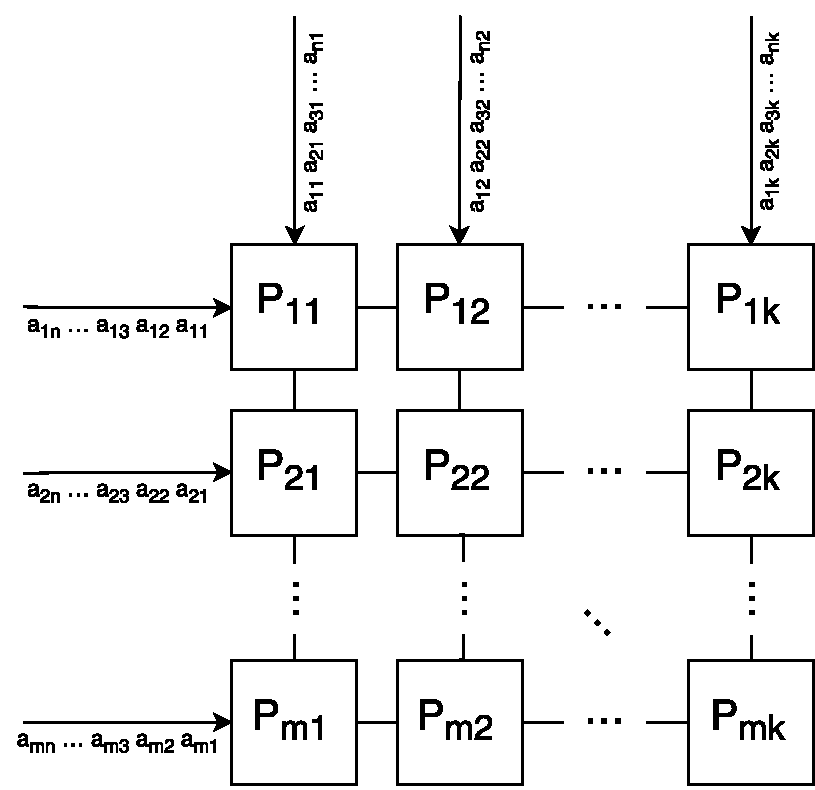
\includegraphics[width=0.5\linewidth]{mesh}
    \centering
	\caption{Schéma zapojení procesorů do mřížky.}
    \label{schema}
\end{figure}

\subsection{Analýza algoritmu}
Nulování registru \textit{C} proběhne v konstatním čase. Poslání prvků $a_{m1}$ a $b_{1k}$ topologicky nejvzdálenějšímu procesoru $P_{mk}$ trvá $m+k+n - 2$ kroků. Pokud předpokládáme, že $m \leq n$ a $k \leq n$, poté algoritmus ma časovou složitost $t(n) = \mathcal{O}(n)$. Pokud budeme uvažovat čtvercové matice, bude algoritmus potřebovat celkem $n^2$ procesorů. Z toho vyplývá celková cena algoritmu $c(n) = \mathcal{O}(n^3)$. To značí, že algoritmus mesh multiplication není optimální.

\section{Implementace}

Při inicializaci program vytvoří $n*k$ procesorů, kde procesor $P_{00}$ řídí vstup a výstup programu, rozesílá načtené matice dalším procesorům a vypisuje výpočítanou matici. Při načítání matice proběhne kontrola, zda je matice v korektním formátů a rozměru. Načtené matice $A$ a $B$ jsou zkontrolovány, zda mohou být vynásobeny a následně jsou jednotlivé řádky matice $A$ poslány na procesory v prvním sloupci a sloupce matice $B$ rozeslány na procesory v prvním řádku. Ty postupně odebírají prvky z fronty a po načtení prvků z obou matic jsou vynásobeny a přičteny k registru $C$.

Všechny procesory jsou informovány o celkových rozměrech obou matic $A$ a $B$ pomocí \textit{broadcast} zpráv. Pokud při kontrole matic dojde k chybě, je tato chyba také distribuována pomocí \textit{broadcast} zprávy.

Dále jsou prvky poslány svým pravým a spodním sousedům. Prvky A svým pravým sousedům a prvky B svým spodním sousedům. Procesory na pravém a spodním okraji po výpočtu prvky zahazují.

Pokud má procesor neprázdné registry $X$ a $Y$, poté při každém přijetí nového čísla $y$ provede porovnání registru $X$ a $Y$ a adekvátně inkrementuje registr $C$. Následně zkontroluje rovnost těchto čísel. Pokud se rovnají, provede kontrolu interně vedeného čítače duplicit čísla $x$. Pokud je těchto duplicit $>1$, porovná index čísla $y$ a rank procesoru a upraví registr $C$ dle algoritmu. Index čísla $y$ je zasílán společně s číslem $y$.

Po dokončení čtení a rozeslání všech čísel procesorem $P_0$ a po přenesení všech čísel skrze lineární spojení jsou asynchronně po sběrnici rozeslány čísla $x$ procesoru s rankem odpovídající hodnotě $c$. Procesory toto číslo uloží do registru $Z$.

Následně jsou čísla z registru poslána svému sousedovi s nižším rankem. Procesor $P_0$ je tiskne na výstup, dokud není vytištěno $n$ čísel. Následuje finalizace programu a ukončení.

\section{Experimentální ověření časové složitosti}

Experimety probíhaly na stroji disponujícím Intel Core i7-2635QM @ 2.00GHz, 8 GB RAM a SSD. Výsledný čas je průměr z 10 měření každého testu. Čas výpočtu byl měřen pomocí Open MPI funkce \texttt{Wtime()}. Z naměřených výsledků je patrné, že do 70 procesorů je výpočet lineární. Při větších počtech procesorů se již projevuje režie fyzického procesoru.

\begin{figure}[!ht]
    \centering
		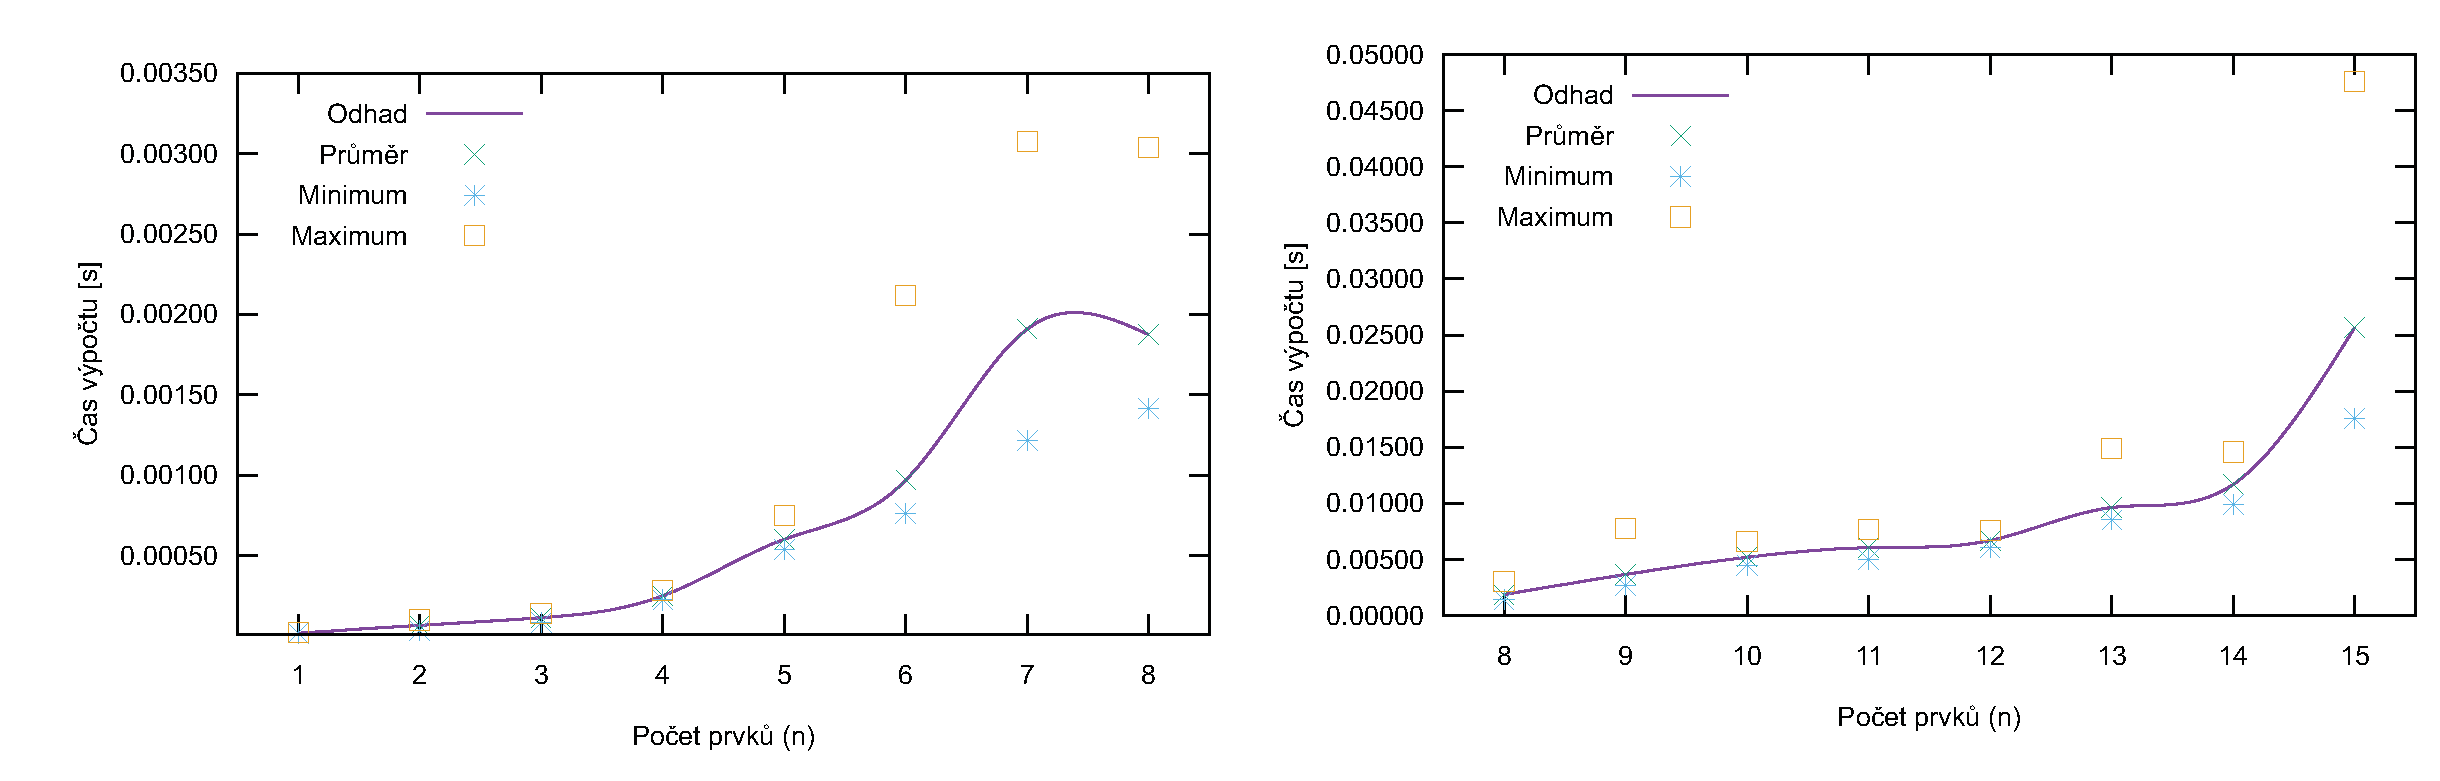
\includegraphics[width=0.6\textwidth]{results}
    \caption{Experimentálně naměřené výsledky}
\end{figure}

\section{Komunikační protokol}
\label{proto}

Protokol je znázorněn na obrázku \ref{proto_schema}. Zasílání zpráv je realizováno výhradně funkcemi \texttt{Send}, \texttt{Isend}, \texttt{Recv} a \texttt{Irecv} z knihovny Open MPI. Tag \texttt{ORD} je pro zasílání indexu čísla $Y$, ostatní tagy slouží k zasílání daných hodnot registrům $X/Y/Z$.

\begin{figure}[!h]
    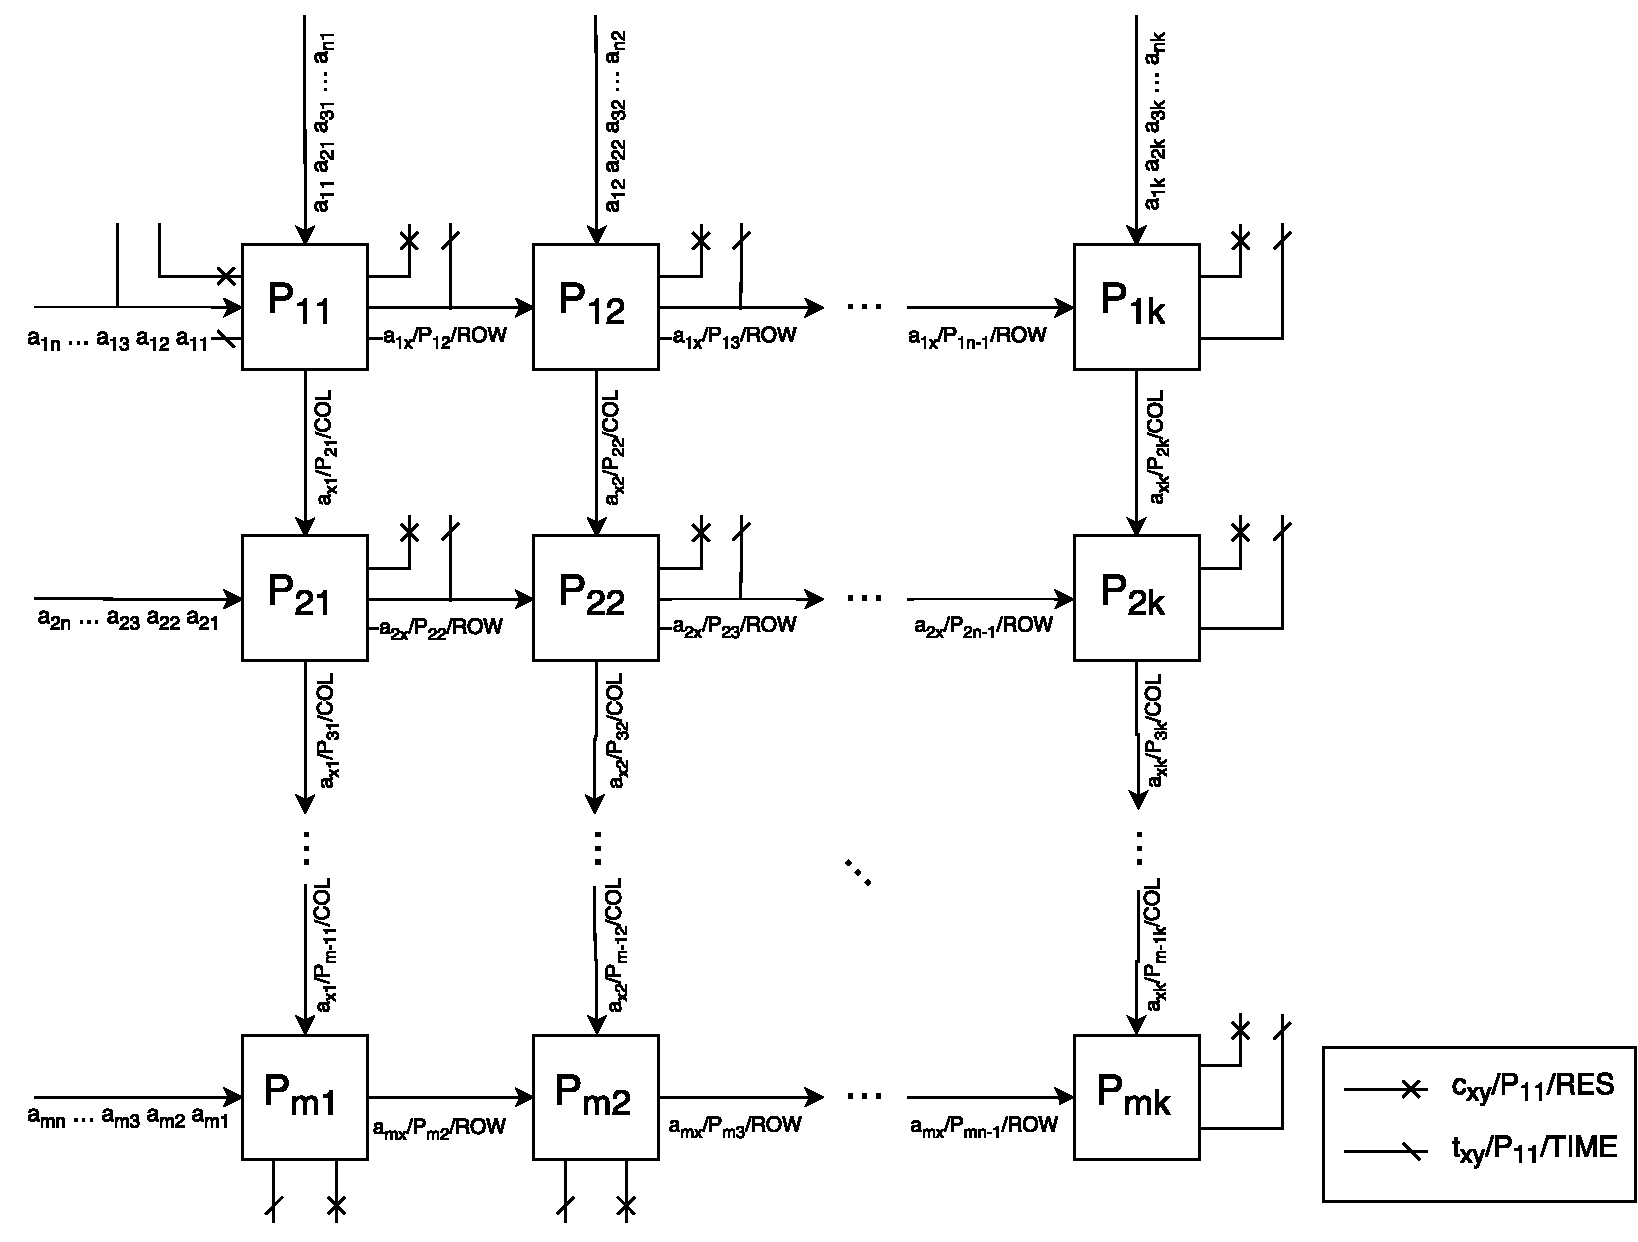
\includegraphics[width=0.8\linewidth]{protokol}
    \centering
    \caption{Sekvenční diagram komunikačního protokolu. Popisky obsahují následující informace: obsah registru, rank, tag.}
    \label{proto_schema}
\end{figure}


\section{Závěr}

Algoritmus se podařilo úspěšně implementovat a experimentálně otestovat. Algoritmus byl upraven tak, aby řadil i duplicitní hodnoty. Z naměřených výsledků lze usoudit, že algoritmus má lineární časovou složitost. Výsledky s více než 70 prvky těmto předpokládům neodpovídají kvůli zvýšené režii při přepínání procesů.


%\bibliography{literature}

%\makeatletter
%\makeatother
%\bibliographystyle{czechiso}

\end{document}

